\section{Context}
%In this section, we introduce concepts needed throughout the rest of the paper. 
%the kNN operation and the MapReduce framework, as well as some needed concepts to compare the existing methods about kNN 
%joins.
\subsection{k Nearest Neighbors}
A nearest neighbors query consists in finding at most $k$ points in a data set $S$ that are the closest to a considered point $r$, in a dimensional space $d$. More formal definitions are as follows: 
%Here we will see some definitions about kNN in this part.
%\TODO{I am not happy with the bunch of definitions here, too many, do we really need all of them?}
given two data sets $R$ and $S$ in $\mathbf{R}^d$, and given $r$ and $s$, two elements, with $r \in R$ and $s \in S$, we have:
%
%\begin{myDef}
%	The \textbf{similarity distance} between any two elements is their distance $d(r,s)$.
%\end{myDef}

\begin{myDef}
	Let $d(r,s)$ be the distance between $r$ and $s$. The \textbf{kNN query} of $r$ over $S$, noted $kNN(r,S)$ is the subset $\{s_i\} \subseteq S$ $\left(\left|\{s_i\}\right| = k\right)$, which is the $k$ nearest neighbors of $r$ in $S$, where $\forall$ $s_i \in kNN(r,S)$, $\forall$ $s_j \in S-kNN(r,S)$, $d(r,s_i) \leq d(r,s_j)$.
\end{myDef}

It is easy to extend the previous definition to a set of query points. 
\begin{myDef}
	The \textbf{kNN join} of two datasets $R$ and $S$, kNN($R$ $\ltimes$ $S$) is:
	\begin{center}
	kNN($R$ $\ltimes$ $S$)=\{($r$,kNN($r$,$S$)), $\forall$ $r \in R$\}
	\end{center}	
\end{myDef}
Depending on the use case, it might not be necessary to find the exact solution of a kNN query, and that is why approximate kNN queries have been introduced. The idea is to have the $k^{th}$ approximate neighbor not far from the $k^{th}$ exact one, as shown in the following definition. 
\begin{myDef}
    The \textbf{$\left(1+\epsilon\right)$-approximate kNN query} for a query point $r$ in a dataset $S$, $AkNN(r,S)$ is a set of approximate $k$ nearest neighbors of $r$ from $S$, if the $k^{th}$ furthest result $s^{k*}$ satisfies $s^{k*} \leq s^k \leq (1+\epsilon)s^{k*} $ $(\epsilon > 0)$ where $s^k$ is the exact $k^{th}$ nearest neighbor of $r$ in $S$.
\end{myDef}

And as with exact kNN, this definition can be extended to an approximate kNN join. 
\begin{myDef}
    The \textbf{$\left(1+\epsilon\right)$-approximate kNN join} of two datasets $R$ and $S$, AkNN($R$ $\ltimes$ $S$) is:
	\begin{center}
	AkNN($R$ $\ltimes$ $S$)=\{($r$,AkNN($r$,$S$)), $\forall$ $r \in R$\}
	\end{center}	    
\end{myDef}


The basic solution to compute kNN adopts a block nested loop approach, which calculates the distance between every object $r_i$ in $R$ and $s_j$ in $S$ and 
sorts the results to find the $k$ smallest. This approach is computational intensive, making it unpractical for large or intricate datasets. Two
strategies have been proposed to work out this issue.  
%To overcome the limitation of this trivial method, many improvements have been done. These improvements can be divided into 2 categories:

The first one consists in reducing the number of distances to compute, by avoiding scanning the whole dataset. This strategy focuses on indexing the 
data through efficient data structures. For example, a one-dimension index structure, the $B^+$-Tree, is used in \cite{DBLP:journals/tods/JagadishOTYZ05} to index distances; 
\cite{MuX} adopts a multipage overlapping index structure R-Tree, whose minimum bound is a rectangle (MBR); \cite{Ciaccia:1997:MEA:645923.671005} 
proposes to use a balanced and dynamic M-Tree to organize the dataset; \cite{Yu:2010:HKJ:1713160.1713227} introduces a sphere-tree with a sphere-shaped minimum bound to reduce the number of areas to be searched; \cite{Andreica13sequentialand} presents a multidimensional quad-tree in order to be able to handle large 
amount of data; and \cite{Bentley:1975:MBS:361002.361007} develops a kd-tree which is a  clipping partition method to separate the search space.

%\end{itemize}

However, reducing the searched dataset might not be sufficient. For data in large dimension space, computing the distance might 
be very costly. That is why a second strategy focuses on projecting the high-dimension dataset onto a low-dimension one, while maintaining the 
locality relationship between data. Representative efforts refer to LSH (Locality-Sensitive Hashing) \cite{Datar:2004:LHS:997817.997857} and 
Space  Filling Curve \cite{5447837}.
In these cases, the low-dimension data contain much less information than the high-dimension ones
because in most cases, the low-dimension data cannot totally fill the high-dimension space. To keep as much information as possible, the trick is to project the high-dimension data multiple times from different perspectives, producing multiple new
datasets.
%\TODO{Done} So these projection methods usually perform multiple operations. 
For instance, LSH usually provides many space hashing functions. The space filling curve method also usually needs several shifts 
of data, to reduce the possibilities of errors in the data locality when projecting. 

But with the increasing amount of data, these methods can still not handle kNN computation 
on a single machine efficiently. Experiments in \cite{10.1371/journal.pone.0044000} suggest using GPUs to significantly improve the 
performance of distance computation, but this is still not applicable for large datasets that cannot reasonably be processed on a single machine. 

%Despite these improvements, large dataset cannot  reasonably be processed on a single machine. 
Recent papers have focused on providing efficient distributed implementations. Some of 
them use ad hoc protocols based on well-known distributed architectures \cite{Novak:2006:MSD:1146847.1146866,Haghani_lshat}. But most of them use the MapReduce model as it is naturally adapted for distributed computation, like in \cite{Stupar10rankreduce-,Lu:2012:EPK:2336664.2336674,Zhang:2012:EPK:2247596.2247602}. In this paper, we focus on the kNN computing systems based on MapReduce, because such systems can scale with the predictable data growth, and also because the framework on which they are based is widespread. 
%\TODO{TODO check phrase}

%
%Since all these improvements have limitations, and these limitations are caused by the amount or the dimension of data, it is indispensable to 
%implement these methods on a parallel and distributed framework such as MapReduce. There have already been some successful works of running kNN on top 
%of MapReduce. Zhang et. al. present an exact and an approximate way of processing kNN on MapReduce in their paper \cite{Zhang:2012:EPK:
%2247596.2247602}. Another similar work was introduced by Lu et. al. in \cite{Lu:2012:EPK:2336664.2336674}. RankReduce \cite{Stupar10rankreduce-} was 
%developed to propose an approach to implement LSH on top of MapReduce. And \cite{Andreica13sequentialand} adapt the well-known sequential algorithms to 
%MapReduce in order to find the nearest neighbors.

%\textit{TODO: definition plus formelle ?}
%The naive way to compute kNN join is, for each point in R to compute the distance from all points in S and keep the k ones for which the distance to the point in R is the smallest. This leads to a complexity O(|R| x |S|) which is not bearable for any real data sets.

\subsection{MapReduce}
MapReduce \cite{Dean:2008:MSD:1327452.1327492} is a parallel programming model that aims at efficiently processing large datasets. This programming 
model is based on three concepts: (i) representing data as key-value pairs, (ii) defining a map function, and (iii) defining a reduce function. 
The map function takes key-value pairs as an input, and produces zero or more key-value pairs. Outputs with the same key are gathered together (shuffled) so that key-\{list of values\} pairs are given to reducers. The reduce function processes all the values associated
with a given key. 
%The overall workflow of a MapReduce computation is shown in Figure~\ref{mapreduce_workflow}.

%\begin{figure*}[htp]
%\center
%\scalebox{0.4}{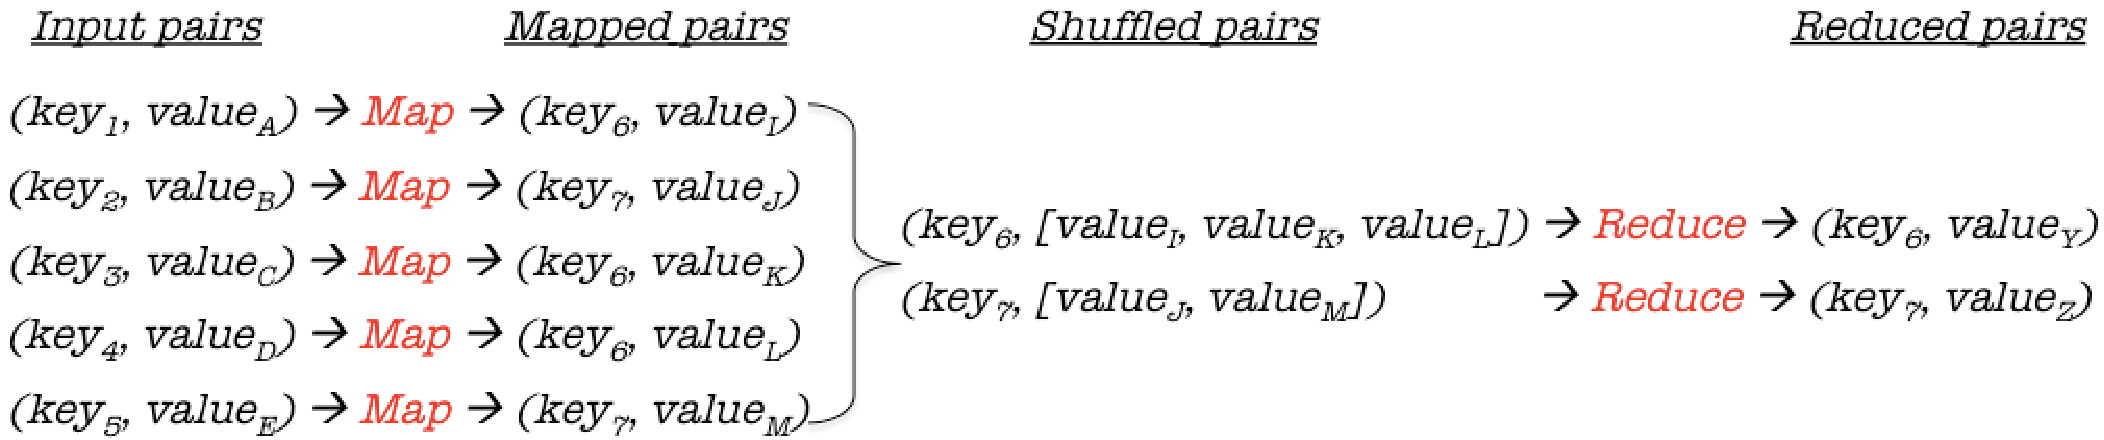
\includegraphics{res/mapreduce.pdf}}
%\caption{MapReduce workflow \label{mapreduce_workflow}}
%\end{figure*}

This decomposition enables data parallelism as the only dependency between the output of the maps and input of reduces. In 
practice, the map and reduce functions can be executed on many machines, leading to a naturally distributed computation. The most famous implementation
of this model is the Hadoop framework \cite{Hadoop:Website} which provides a distributed platform for executing MapReduce jobs. 
%This programming model is based on a representation of data as key-value pairs and on consecutive call of the map and reduce functions, that take as 
%parameter key-value pairs and that also return key-value pairs. The user of the framework has to provide the data format, and the body of the map and 
%reduce functions. The framework then handle parallel and join phases. Typically, massive map tasks (called Mapper) are triggered in parallel according 
%to the data format provided whereas reduce tasks (called Reducer) will gather and then process Mapper's output that have the same key to produce the 
%final output, as can be seen in Figure~\ref{mapreduce_workflow}. 

%\textit{- Distribution:} Many implementations of the MapReduce programming model are adapted to distribution, such as the Hadoop framework 
%\cite{Hadoop:Website}. Indeed, mappers usually process subsets of data that are independent from each other. It is thus natural to distribute mappers 
%across a set of machines, thereby scaling to terabytes of data to process. 

%\TODO{Not sure we need this, we have already justified the paper in the introduction. I suggest removing it}.
%In the context of this paper, using MapReduce to compute kNN join is 
%challenging in the sense that, to be efficient, the kNN query must be run for each point on a subset of the data rather than on the whole data set. It 
%is also a requirement to be compliant with the MapReduce model, since each part of the computation should be independent from each other. We will thus 
%review existing partitioning techniques to do that in the context of MapReduce, and also broader.